%!TEX root = ../MasterThesis.tex

\section{E-commerce Scenario}
\label{sec:e_commerce_scenario}

\textbf{E-commerce} as a term relates to the trading of products or services utilizing a computer network such as the Internet. It is usually categorized into the following four different subfields \citep{sen2015study}:\@

\begin{enumerate}
  \item \textbf{Business-To-Business (\gls{B2B})}: refers to electronic trading between companies with the objective to improve their supply chain processes
  \item \textbf{Business-To-Consumer (\gls{B2C})}: refers to electronic trading between a company and it's consumers (most publicly known example for it is Amazon.com)
  \item \textbf{Consumer-To-Consumer (\gls{C2C})}: refers to electronic trading between consumers (most publicly known example for that is eBay)
  \item \textbf{Consumer-To-Business (\gls{C2B})}: referes to electronic trading between consumers and businesses (most publicly known example for this is TaskRabbit)
\end{enumerate}

This Master thesis will \textbf{\underline{solely}} focus on the \textbf{\gls{B2C}} aspect of E-commerce. In that case a \textbf{consumer} is using an \textbf{E-commerce shop} of a \textbf{merchant} on the Internet to order products or services online. The merchant is offering a catalog of available products or services on the Web, that is available and accessible by the general public and usually has an at least nation-wide if not global reach. The merchant can either run the E-commerce shop software on her own servers (on-premise) or can outsource this additional sales channel to a 3$^{rd}$ party hosting company or \textbf{cloud service provider (\gls{CSP})}. Also the E-commerce shop software itself can either be developed by the merchant in-house or acquired as a boxed product from an \textbf{Independent Software Vendor (\gls{ISV})} on the market. For business accounting purposes the merchant also runs a bank account with the \textbf{acquirer} (see Figure~\ref{fig:images_ecommerce_scenario}). \\

When placing an order with the merchant online the consumer is normally using a \textbf{credit card} for finalizing the transaction. This credit card has originally been handed out by the \textbf{issuing bank} to the consumer. Additionally some online shops make it mandatory for the consumer to create an user account with them while others do not. The former is the preferred way when consumers are repetitively buying from that merchant, whereas the latter might be used for one-time or irregular shopping trips online. To be able to connect to the Internet the consumer also relies on a service of an \textbf{Internet Service Provider (\gls{ISP})}. The whole initial setup for participating on E-commerce activities is found in Figure~\ref{fig:images_ecommerce_scenario}.\@

\begin{figure}[H]
	\centering
		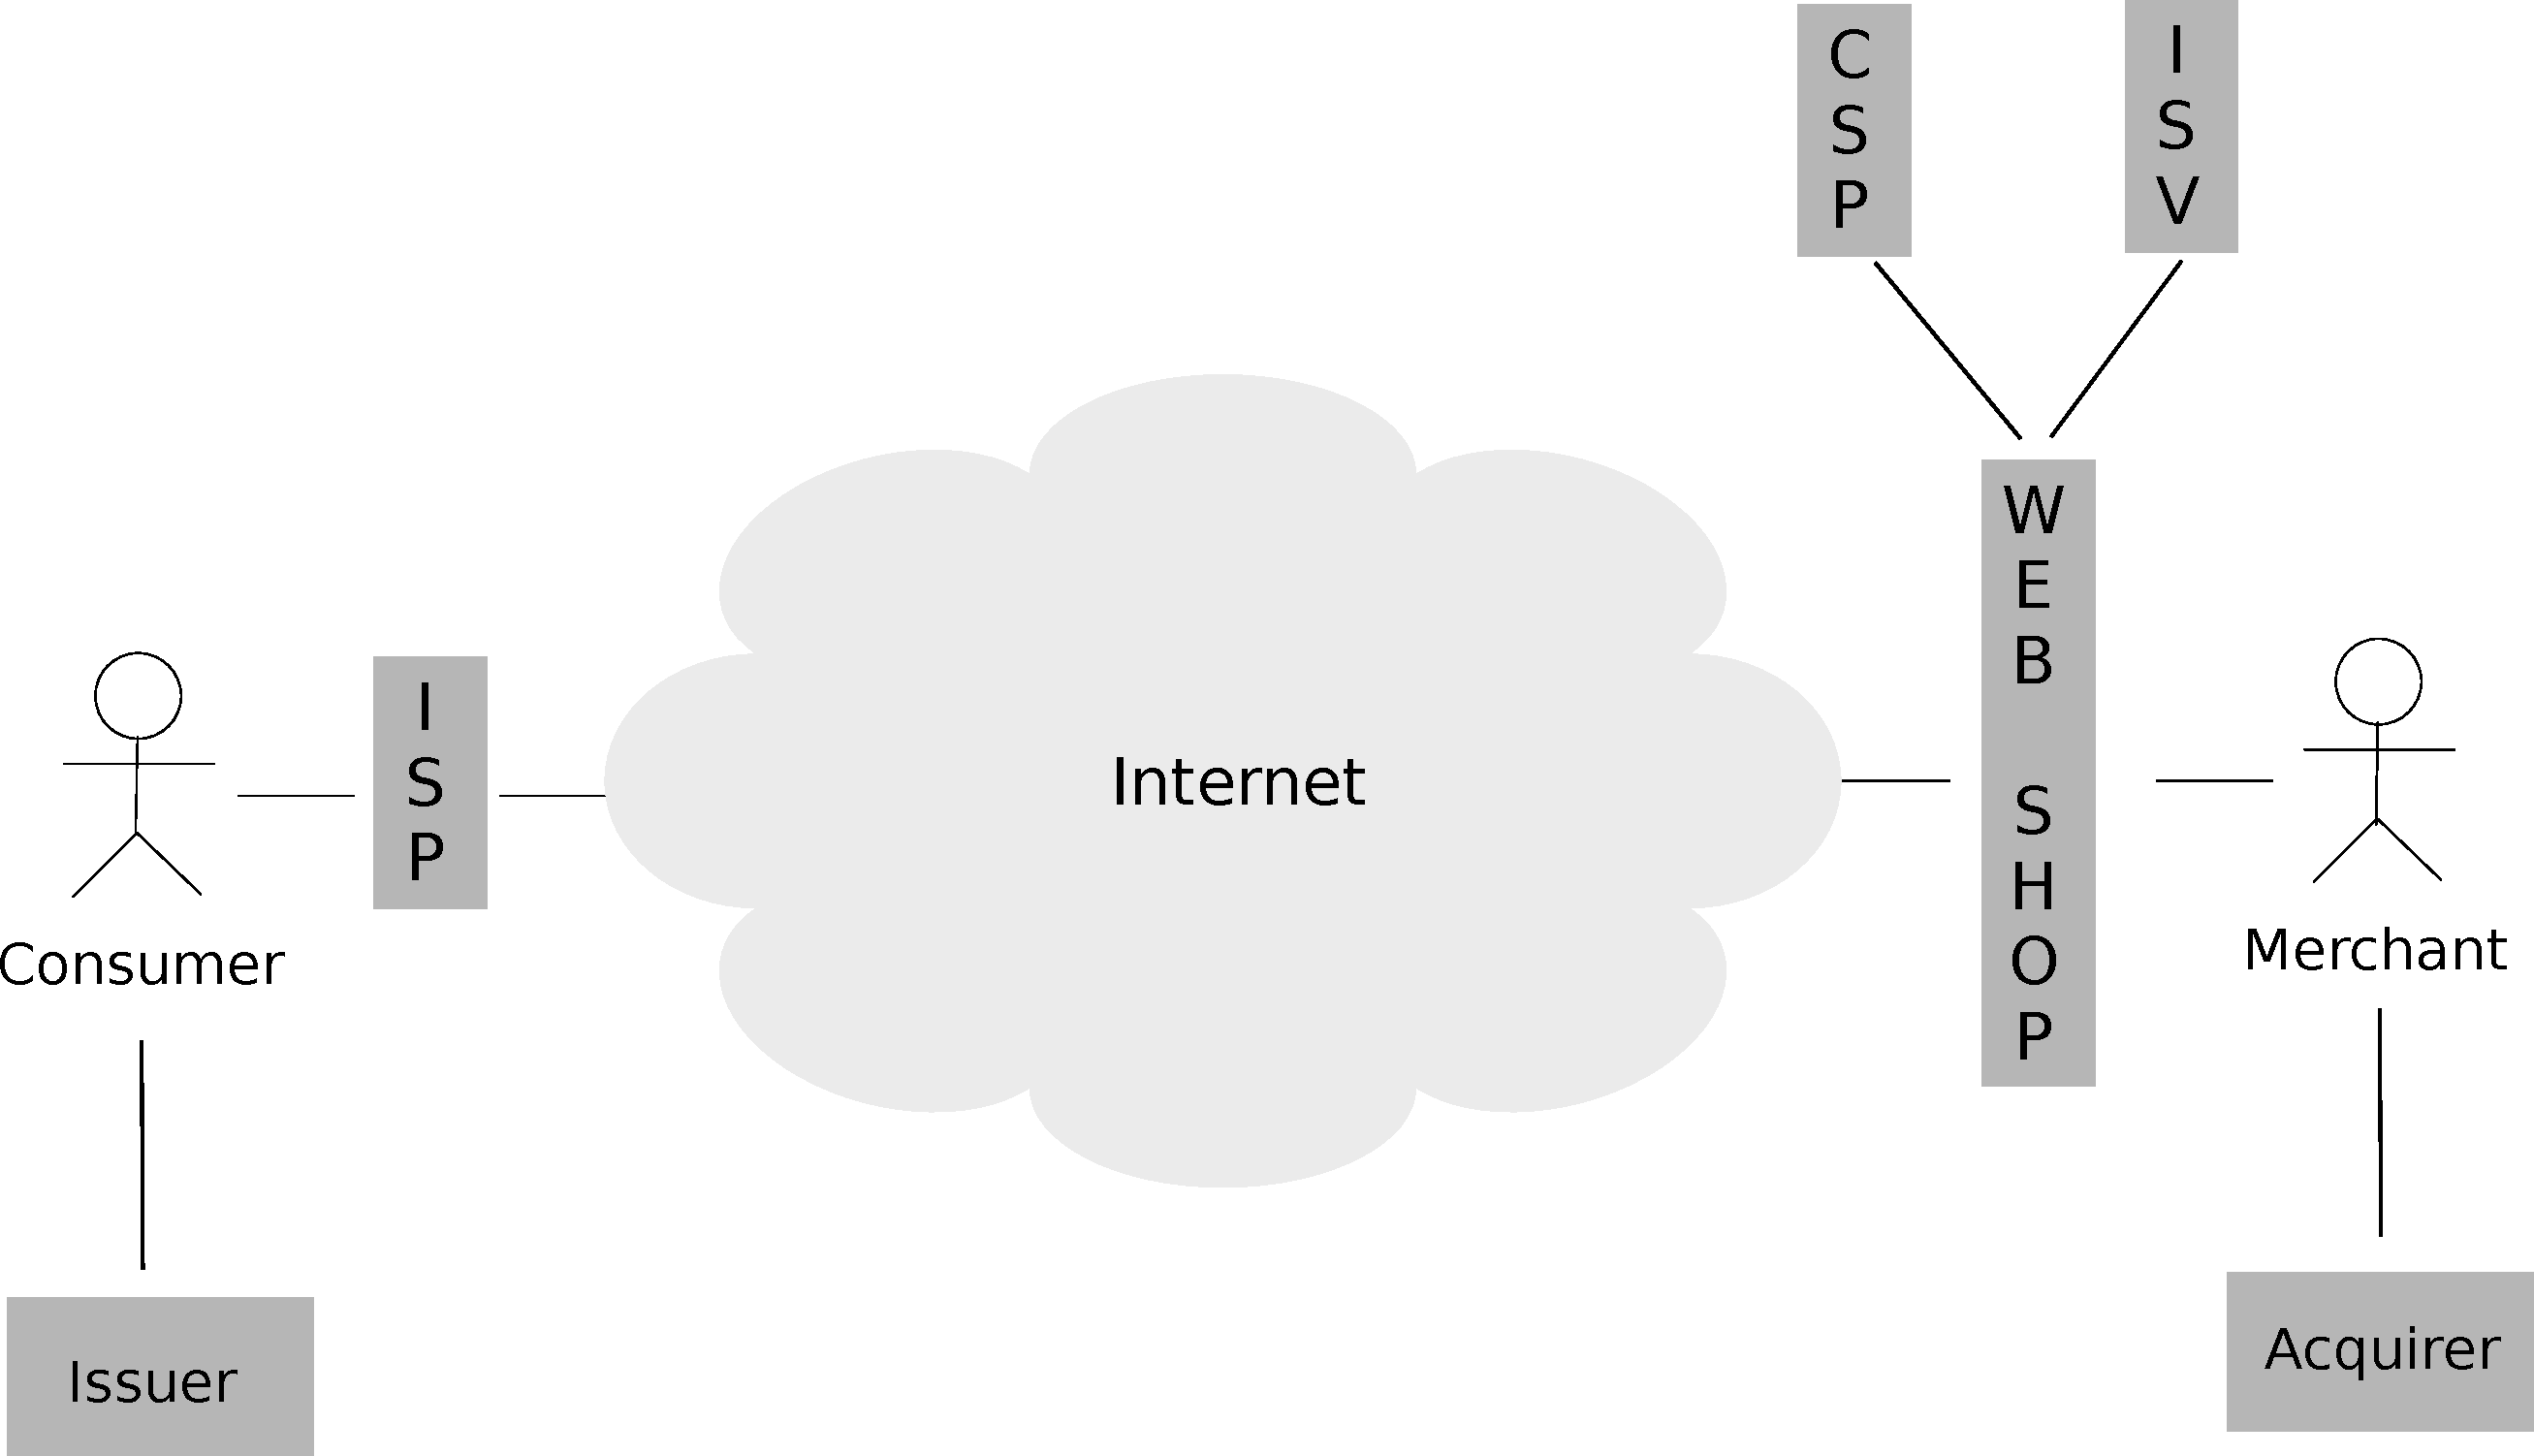
\includegraphics[width=0.8\columnwidth]{images/e-commerce-scenario.pdf}
	\caption{E-commerce Fundamentals}
\label{fig:images_ecommerce_scenario}
\end{figure}

When the consumer places the \textbf{order} online, the merchant receives at least a \textbf{list of products or services} from the current shopping cart of the consumer, the \textbf{identification} of the consumer as well as the \textbf{delivery address} to ship the physical items to. If the transaction is going to be finalized with a credit card, the consumer will have to provide additional information like her \textbf{billing address} and \textbf{credit card information} (including the credit card number, the expiry date and the security number of the card). \\

The merchant usually does not validate the credit card information on her own. For that purpose she is relying on another 3$^{rd}$ party service offered on the Internet by the \textbf{Payment Service Provider (\gls{PSP})}. These providers are either validating the credit card information themselves based on an user profile the consumer has with the \gls{PSP} (e.g.\ a global available Web service offering like PayPal) or are connecting to the issuing bank of the card for doing so. For this validation process the merchant is handing over the following information to the \gls{PSP}:\@

\begin{itemize}
    \item consumer's billing address
    \item given credit card number, expiry date and security number
    \item identification of the merchant
    \item final amount of the transaction actually being processed
\end{itemize}

Either the \gls{PSP} or the issuing bank is validating the correctness of the information with criterias like: \@

\begin{itemize}
    \item is the billing address matching the current consumers' postal address on file?
    \item is the stated credit card information correct and is this credit card not marked as being blocked?
\end{itemize}

The merchant will receive the \textbf{status} of the authorization as well as a \textbf{payment token} in return. If the authorization was done successfully the merchant will collect the items and send out a shipping request to one of the available \textbf{Logistic Service Providers (\gls{LSP})} capable to handle the order. They will pickup the order at the merchant's facility and ship it to the delivery address stated by the consumer. Usually in parallel the merchant is informing her bank about the order, amount due as well as payment token from the \gls{PSP}. The acquirer is in charge to withdrawal the amount of the order from the consumer's bank account either via the \gls{PSP} or directly from the issuing bank, depending on who of them has authorized the initial payment request (a process called clearing) \citep{VisaPayment2014}. The sequence of activities within an E-commerce checkout process is visualized in Figure~\ref{fig:images_ecommerce_checkout_process}.\@

\begin{figure}[H]
	\centering
		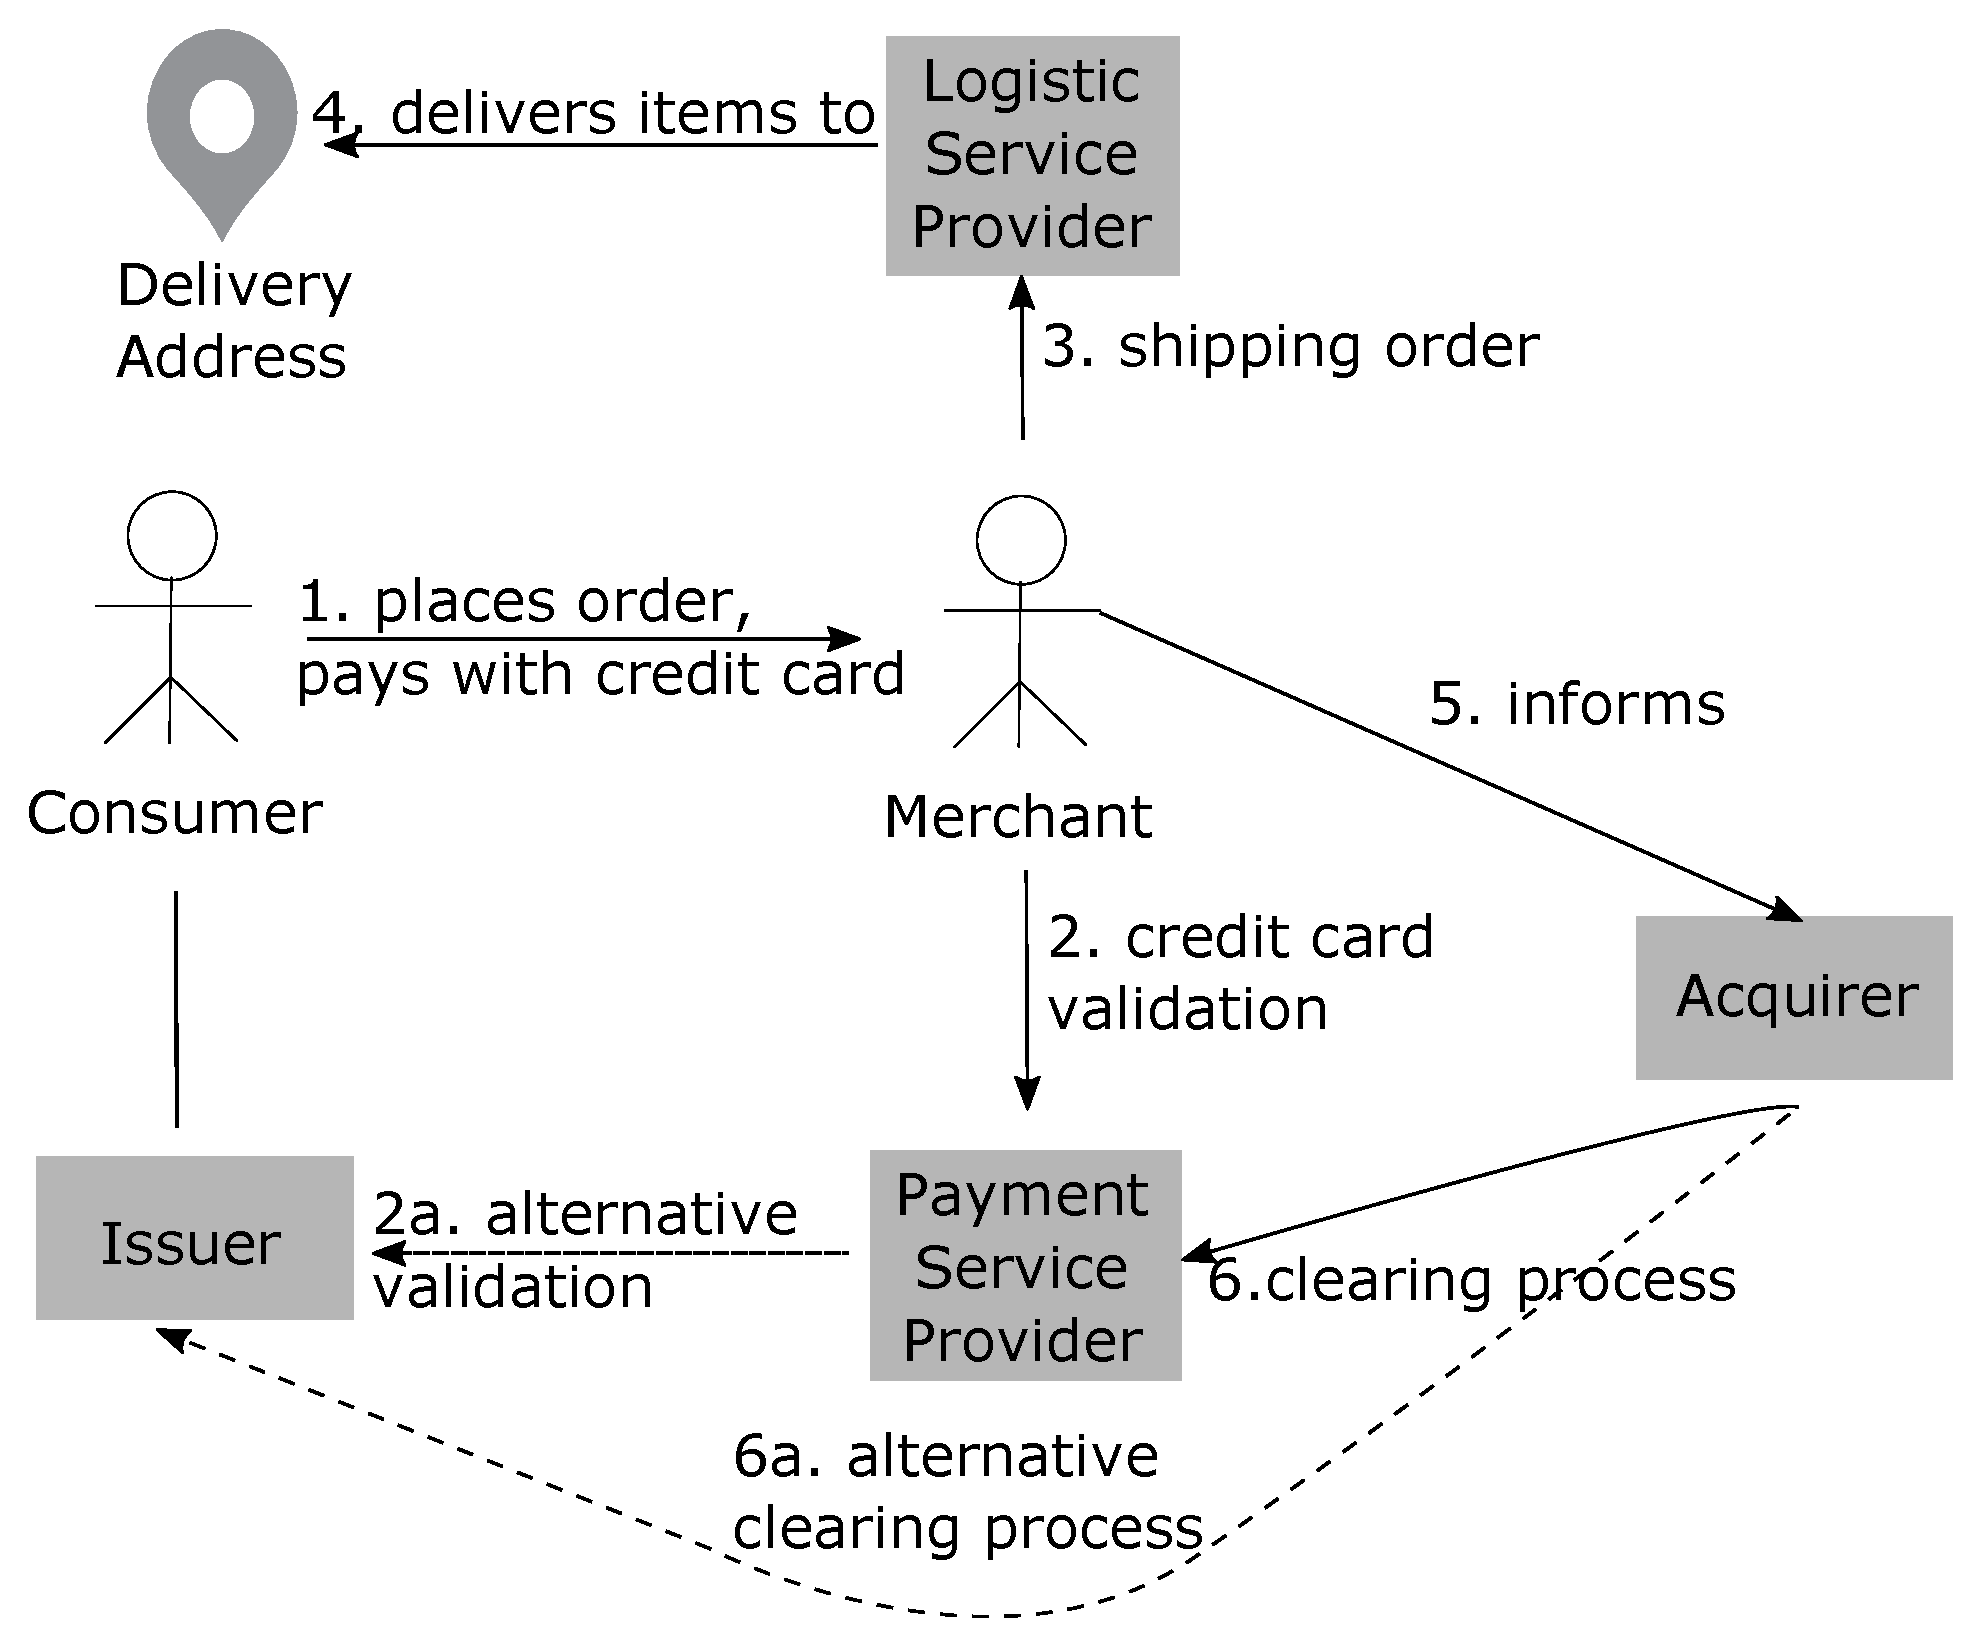
\includegraphics[width=0.8\columnwidth]{images/e-commerce-checkout-process.pdf}
	\caption{E-commerce Checkout Process in detail}
\label{fig:images_ecommerce_checkout_process}
\end{figure}

% section scenario description (end)
